\documentclass{beamer}

\usepackage{graphicx}
\usepackage{framed}

\begin{document}
	%===========================================================%
	\begin{frame}
		\frametitle{Testing the Assumption of Normality}
		\Large
\textbf{	Testing the Assumption of Normality}
	
	\begin{itemize}
		\item	One of the assumptions of many statistical procedures (including the \textbf{t-test}) is that the population from which you are sampling is normally distributed. 
		\item	The t-test is said to be rather ‘\textbf{robust}’ in terms of this assumption, which means that reality can deviate from this assumption a fair amount without seriously affecting the validity of the analysis. 
		\end{itemize}
		
	\end{frame}
	
	
	%===========================================================%
	\begin{frame}
		\frametitle{Testing the Assumption of Normality}
		\Large
		
		\begin{itemize}	
		
		\item This is particularly true when the size of the samples is large (thanks to the Central Limit Theorem). 
		\item Some deviations from normality can pose a problem for the t-test, specifically those that involve getting extreme scores more frequently than you would if the distribution were normally distributed.
	\end{itemize}

	\end{frame}
	
	
	%===========================================================%
	\begin{frame}
		\frametitle{Testing the Assumption of Normality}
		\Large
		\noindent \textbf{Using Computer Software}
		\begin{itemize}
				\item	Statistical Software Packages provides two statistical tests for deviation from normality, the ``Kolomogorov-Smirnov" family of tests and the ``Shapiro-Wilk" test.
				\item	The 'Kolomogorov-Smirnov' test can be used to test if two data sets are distributed according to the same distribution. 
				\item	It can also be used to test if one data set comes from a specified distribution, such as the normal distribution. 
		\end{itemize}

	\end{frame}
	
	
	%===========================================================%
	\begin{frame}
		\frametitle{Testing the Assumption of Normality}
		\Large
		\begin{itemize}
	%		\item	( As such, the normal distribution must be specified as an argument to the function.)
	\item	For the purposes of this module, we will only use a special case of the 'Kolomogorov-Smirnov' test, known as the ``\textbf{Anderson-Darling}" test of normality.
	\item The Shapiro-Wilk Test can be implemented using the \texttt{shapiro.test()} command in \texttt{R}.
	\end{itemize}
\end{frame}


%===========================================================%
\begin{frame}
	\frametitle{Testing the Assumption of Normality}
	\Large	
	\textbf{Implementing the Tests}
	\begin{itemize}	\item	The ``Anderson-Darling" test can not be implemented immediately with \texttt{R}. 

			\item Using the Anderson Darling Test requires the installation of the \textbf{nortest} package. 
			\item Then the test can be implemented using the \texttt{ad.test()} command.
			\item (There are actually more procedures. We will look at R packages in greater detail on an ongoing basis.)
	\end{itemize}
\end{frame}


%===========================================================%
\begin{frame}
	\frametitle{Testing the Assumption of Normality}
	\Large	
	\textbf{Implementing the Tests}
	\begin{itemize}
					\item	\alert{IMPORTANT} The null hypothesis of both the `\textbf{Anderson-Darling}’ and `\textbf{Shapiro-Wilk}’ tests is that the population, from which the sample is drawn, is normally distributed 
			\item The alternative hypothesis is that the population, from which the sample is drawn, is not normally distributed.
			
			\end{itemize}
			
		\end{frame}
				
		%===========================================================%
		\begin{frame}
			\frametitle{Testing the Assumption of Normality}
			\Large	
			\textbf{Implementing the Tests}
			\begin{itemize}		
			\item	Let us use both tests to assess whether an example data set is normally distributed. (This data set is one that we are going to use in Lab Classes later on) 
			\item	Judging by this histogram on the next slides – do you think the data set is normally distributed?
		\end{itemize}

	\end{frame}
	
	
	%===========================================================%
	\begin{frame}
		\frametitle{Testing the Assumption of Normality}
		\Large
		\begin{figure}
\centering
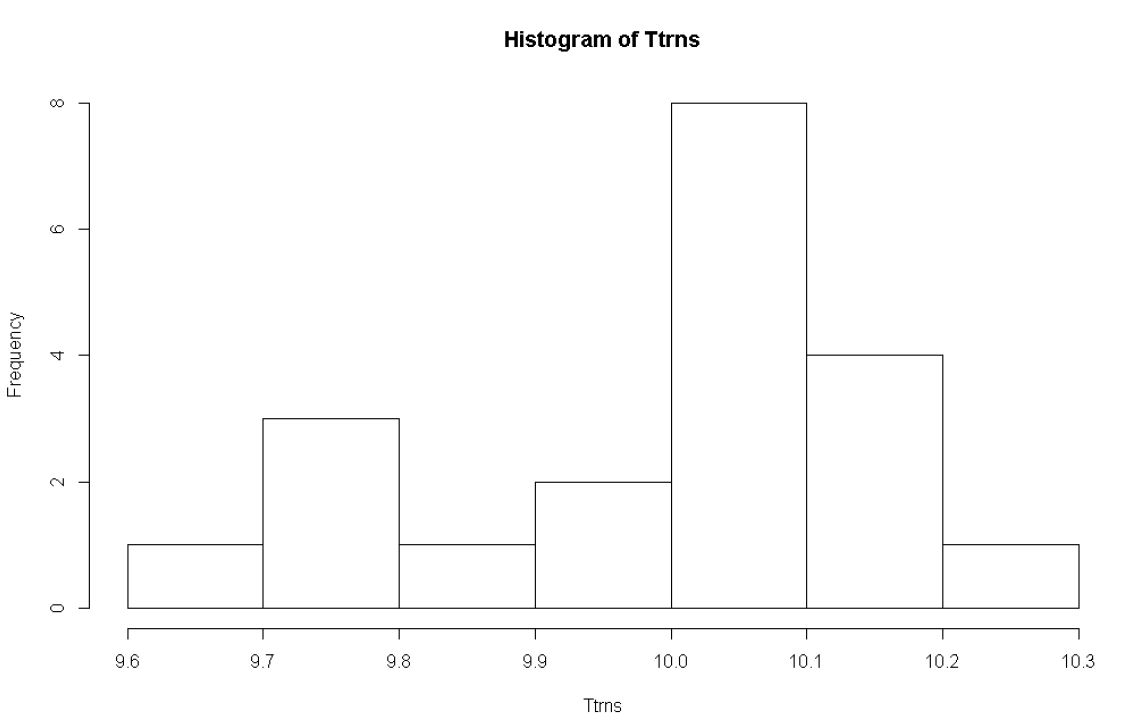
\includegraphics[width=1.1\linewidth]{images/Histogram1}
\end{figure}
(Remark : it is skewed to the right)
\end{frame}
%===========================================================%
\begin{frame}
\frametitle{Testing the Assumption of Normality}
\Large	
\textbf{Using the Shapiro-Wilk Test}		
\begin{figure}
\centering
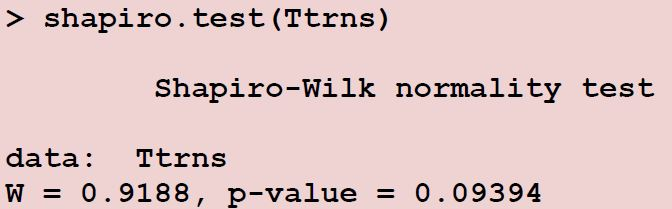
\includegraphics[width=0.9\linewidth]{images/ShapiroTestR1}
\end{figure}
\end{frame}
%===========================================================%
\begin{frame}
\frametitle{Testing the Assumption of Normality}
\Large	
\textbf{Using the Anderson Darling Test}	
\begin{figure}
\centering
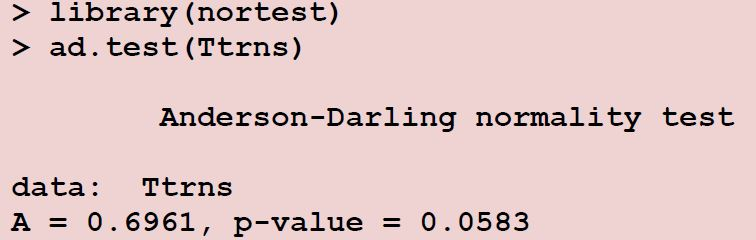
\includegraphics[width=0.9\linewidth]{images/ADtestR1}

\end{figure}

			
		\end{frame}
	%===========================================================%
	\begin{frame}
		\frametitle{Testing the Assumption of Normality}
		\Large
	\textbf{Conclusion}
	\begin{itemize}
	\item	In both cases we fail to reject the null hypothesis that the data set is normally distributed.
  \item Just to clarify, we are not explicitly stating that the population, from which the sample is drawn, is Normally Distributed. (See next section.)
	\end{itemize}
	\end{frame}
	
	%===========================================================%
	\begin{frame}
		\frametitle{Testing the Assumption of Normality}
		\Large	
	
	
		 
		\textbf{Limitations of Tests}
		\begin{itemize}
		\item	There are some important limitations to the usefulness of these tests. 
		\item	If you reject H$_0$ you can conclude that the population is not normally distributed, but if you don't reject H$_0$ then you only conclude that you failed to show the population is not normally distributed. 
		\item	In other words, you can prove the population is not normally distributed but you can't prove it is normally distributed. 
			\end{itemize}
		\end{frame}
		%===========================================================%
		\begin{frame}
			\frametitle{Testing the Assumption of Normality}
			\Large		
			\textbf{Limitations of Tests}
			\begin{itemize}	
					\item	Rejecting H$_0$ means that the population is not normally distributed, but it doesn't tell you whether it is because it is a fat-tailed distribution, a thin-tailed distribution, a skewed distribution, or something else.
		\item	Also - the tests are influenced by power. If you have a small sample the test may not have enough power to detect non-normality in the population.
		\end{itemize}
	\end{frame}
	%===========================================================%
	\begin{frame}
		\frametitle{Testing the Assumption of Normality}
		\Large		
	\textbf{Q-Q plot}
	\begin{itemize}	
	\item	The quantile-quantile (Q-Q) plot is an excellent way to see whether the data deviate from normal.
	\item	The process used for creating a QQ plot involves determining what proportion of the 'observed' scores fall below any one score. 
	\item	Then the “z- score” that would fit that proportion if the data were normally distributed is calculated,
			\end{itemize}
		\end{frame}
		%===========================================================%
		\begin{frame}
			\frametitle{Testing the Assumption of Normality}
			\Large		
			\textbf{Q-Q plot}
			\begin{itemize}		\item	Finally that “z- score” that would cut off that proportion (the `expected normal value') is translated back into the original metric to see what raw score that would be. 

				\item	A scatter plot is then created that shows the relationship between the actual `observed' values and what those values would be `expected' to be if the data were normally distributed. 
			\end{itemize}
		\end{frame}
		%===========================================================%
		\begin{frame}
			\frametitle{Testing the Assumption of Normality}
			\Large		
			\textbf{Interpreting Q-Q plots}
			\begin{itemize}	
				\item	If the data is normally distributed then the circles on the resulting plot (each circle representing a score) will form a straight line. 
	\item	A trend line can be added to the plot to assist in determining whether or not this relationship is linear.
	\end{itemize}
		\end{frame}
		%===========================================================%
		\begin{frame}[fragile]
			\frametitle{Testing the Assumption of Normality}
			\Large		
			\textbf{Implenting Q-Q plots in \texttt{R}}
	
	\begin{framed}
	\begin{verbatim}
	> qqnorm(Ttrns) 
	> qqline(Ttrns)
	\end{verbatim}
	\end{framed}
How well do the covariates follow the trendline? Compare your conclusion to the  p-values of the formal tests.
			\end{frame}
			%===========================================================%
			\begin{frame}
				\frametitle{Testing the Assumption of Normality}
				\Large		
\begin{figure}
\centering
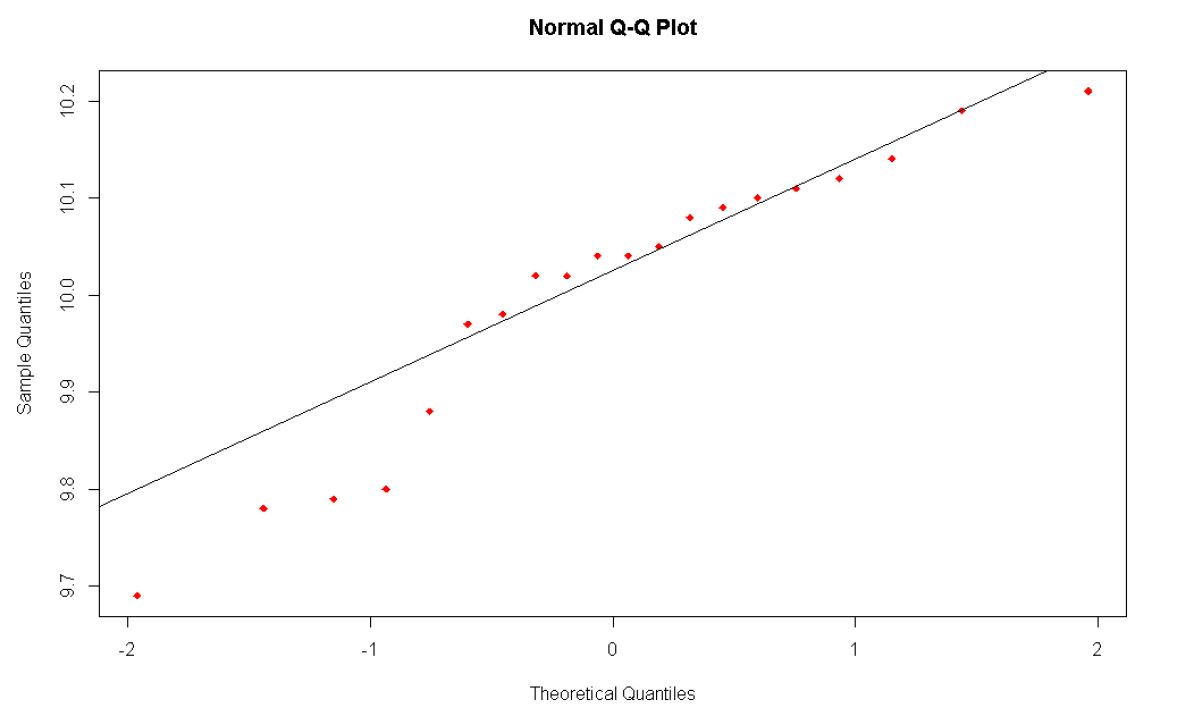
\includegraphics[width=1.1\linewidth]{images/QQplot1}

\end{figure}
\end{frame}
	%===========================================================%		
\begin{frame}
\large
	\textbf{Interpreting Q-Q plots}\\ 
\begin{itemize}
	\item Most of the points follows the trend-line, but there are several observations that are fairly fair far away in the bottom left
	\item We will look at transformations next class
\end{itemize}
		\end{frame}
	%===========================================================%			
	\begin{frame}
		\textbf{Interpreting Q-Q plots}\\ 
\begin{itemize}
\item This is the QQplot for an unseen data set.
\item Conclusion : Safe to assume normal distribution, despite some outliers
\end{itemize}
		\begin{figure}
\centering
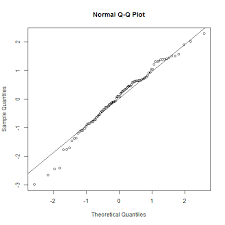
\includegraphics[width=0.55\linewidth]{images/qqnormal}

\end{figure}
	%===========================================================%	
	\end{frame}
		\begin{frame}
		\textbf{Interpreting Q-Q plots}\\ Assumption of normal distribution clearly not valid in these cases
\begin{figure}
\centering
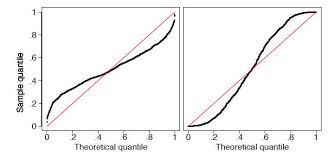
\includegraphics[width=0.9\linewidth]{images/qqnotnormal1}

\end{figure}
			
		\end{frame}
	%===========================================================%	
			\begin{frame}
					\textbf{Interpreting Q-Q plots}\\ Assumption of normal distribution clearly not valid in this case.
			\begin{figure}
				\centering
				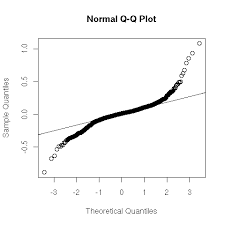
\includegraphics[width=0.7\linewidth]{images/qqnotnormal2}

			\end{figure}
			
		\end{frame}		
		%===========================================================%
\begin{frame}
	\Large
\textbf{Review}
\begin{itemize}
	\item Know the null and alternative hypothesis for formal hypothesis tests for normality.
	\item Be able to interpret R code output.
	\item Discuss the limitations of these tests
	\item Know how to interpret Q-Q plots (in conjection with formal tests)
 \item (Some material will be added when we get to Statistical Process Control Section.)
\end{itemize}
\end{frame}
\end{document}